\section{Introduction} 

\begin{figure}[t] \begin{center}
    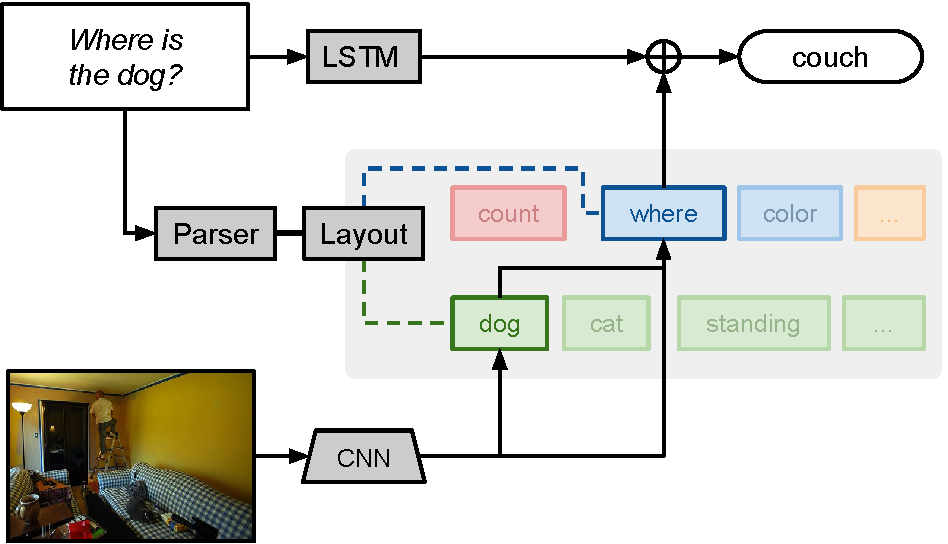
\includegraphics[width=\linewidth]{fig/teaser} \end{center} \caption{
      A schematic representation of our proposed model---the shaded gray area is a
      {\it neural module network} of the kind introduced in this paper. Our
      approach uses a natural language parser to dynamically lay out a deep
      network composed of reusable modules. For visual question answering tasks,
      an additional sequence model provides sentence context and learns
      common-sense knowledge.
    } \label{fig:teaser}
\end{figure}

This paper describes \emph{neural module networks} (NMNs), a modular framework
for visual quesiton answering. We answer natural language questions about images
using collections of jointly-trained neural ``modules'', dynamically assembled
into deep networks based on linguistic structure. 

The visual QA task has been the subject of a great deal of recent research
attention
\cite{antol15iccv,gao2015you,ma15arxiv,malinowski15iccv,ren2015image,yu15arxiv},
and has significant applications to human-robot interaction, search, and
accessibility.  Visual QA requires sophisticated understanding of both visual
scenes and natural language.
%
Concretely, given an image and an associated question (e.g.\ \emph{where is
the dog?}), we wish to predict a corresponding answer (e.g.\ \emph{on the
couch}, or perhaps just \emph{couch}). Recent successful approaches represent
questions as bags of words, or encode in the question using a recurrent neural
network \cite{malinowski15iccv} and train a simple classifier on the encoded
question and image. In contrast to these monolithic approaches, another line of
work for textual QA \cite{Liang13DCS} and image QA \cite{malinowski14nips} uses
semantic parsers to decompose questions into logical expressions. These logical
expressions are evaluated against a purely logical representation of the world,
which may be provided directly or extracted from an image
\cite{Krish2013Grounded}.

In this paper we draw from both lines of research, presenting a technique for
integrating the representational power of neural networks with the flexible
compositional structure afforded by symbolic approaches to semantics.  Rather
than relying on a monolithic network structure to answer all questions, our
approach assembles a network on the fly from a collection of specialized,
jointly-learned modules (\autoref{fig:teaser}). Rather than reasoning over
truth values, we remain entirely in the domain of visual features and
attentions.

Our approach first analyzes
each question with an off-the-shelf semantic parser, and uses this analysis to
determine the basic computational units (attention, classification, etc.) needed
to answer the question, as well as the relationships between the modules. In
\autoref{fig:teaser}, we first produce an attention focused on the dog, which
passes its output to
a location classifier. Depending on the underlying structure, these messages
passed between modules may be raw image features, attentions, or classification
decisions; each module is determined by its input and output types.
Different kinds of modules are shown in different colors; attention modules
(like \mod{dog}) are shown in green, while labeling modules (like
\mod{where}) are shown in blue.
%Different kinds of modules are marked with different
%colors in \Figref{fig:teaser}: for example the \mod{attend[$dog$]} module
%(green) produces a spatial heatmap while the \mod{classify[$where$]} (blue)
%recognizes what is in the image region localized by the attention heatmap.
Importantly, all modules of a NMN are independent and composable, which allows
the computation to be different for each problem instance, and possibly
unobserved during training. 
%So that we can answer novel question at test time, such as
%\emph{Where is the banana?}, even we only saw \emph{count} or
%\emph{color} question about \emph{bananas} during training.  
Outside the NMN, our final answer incorporates the image scene knowledge
(using a full frame CNN) and uses a recurrent network (LSTM) to read the
question, which has been shown to be important to model common sense knowledge
and dataset biases \cite{malinowski15iccv}.

%Where previous work has
%treated both the image and the question as inputs to a monolithic
%classification model, we instead take the perspective that a question is a
%noisy specification of a hidden computation that must be performed on the image
%to produce an answer. Crucially, this computation may be different for each
%problem instance, and is never observed observed during training.

%Our approach bears a superficial resemblance to a classical semantic parser.
%However, instead of mapping from questions to logical forms, our model maps
%from questions to neural network structures. These networks are assembled on
%the fly (possibly into novel topologies) from a collection of jointly-learned
%neural ``modules''. Finally, they are evaluated against the input image to
%produce an answer.




%This paper presents a technique for following natural language instructions
%(and performing other dynamically-specified tasks) by assembling deep neural
%networks on the fly from an inventory of pre-trained components.

We evaluate our approach on three visual question answering tasks. On the
recently-released CocoQA \cite{yu15arxiv} and VQA \cite{antol15iccv} datasets,
we achieve results comparable to or better than existing approaches, and show
that our approach specifically outperforms previous work on questions with
compositional structure (\eg requiring that an object be located and one of its
attributes described). It turns out, however, that many of the questions in both
datasets are quite simple, with little composition or reasoning required. To
test our approach's ability to handle harder questions, we introduce
a new dataset of synthetic images paired with complex questions involving
spatial relations, set-theoretic reasoning, and shape and attribute recognition.
On this dataset we outperform competing approaches by as much as 25\% absolute
aaccuracy.

While all the applications considered in this paper involve visual question
answering, the general architecture is potentially of broader usefulness, and
might be more generally applied to visual referring expression resolution (XXX)
or question answering about natural language texts (XXX).

%We evaluate our approach on two visual question answering tasks. First we
%present a new synthetic image dataset paired with a complex set of queries
%(involving spatial relations, logical operators, and shape and attribute
%recognition). Next, we consider a hard subset of the Microsoft VQA corpus of
%questions about natural images. In each case, an NMN-based approach outperforms
%state-of-the-art models with more conventional recurrent architectures. We
%observe in particular that NMNs are able to make considerably better use of
%small training sets.

To summarize our contributions: We first describe neural module networks, a
general architecture for discretely composing heterogeneous, jointly-trained
neural modules into deep networks. Next, for the visual QA task specifically, we
show how to construct NMNs based on the output of a semantic parser, and use
these to successfully complete established visual question answering tasks.
Finally, we introduce a new dataset of challenging, highly compositional
questions about abstract shapes, and show that our model again outperforms
previous approaches. We will release this dataset, as well as code for all
systems described in this paper, upon publication.

\section{Motivations}

%Many tasks in computer vision, including recognition, detection, and captioning,
%share common substructure. For example, we might schematically express the
%sequence of computations performed by a recognizer as
%\begin{flushleft}
%  \mod{classify(pickMostRelevant(detectObjects))}
%\end{flushleft}
%or a detector as
%\begin{flushleft}
%  \mod{drawBoundaries(detectObjects)}
%\end{flushleft}
%
%In practice the picture is not this clean---classification or detection is
%performed end-to-end by a single neural network, and the boundaries between
%these ``phases'' are not clearly defined. Nevertheless we might expect \textit{a
%priori} that a network used for classification might expose intermediate
%representations useful for building a detector. 
We begin with two simple observations. First, that there is no single ``best
network'' for all purposes---state-of-the-art performance on the full range of
computer vision tasks that are studied requires a variety of different deep
network topologies. Second, though different networks are used for different
purposes, it is commonplace to initialize systems for many of vision tasks with
a prefix of a network trained for classification \cite{Long14FullyConvolutional} XXX. 
This has been shown to substantially reduce training time and improve accuracy. 

So while network structures are not \emph{universal} (in the sense that the same
network is appropriate for all problems), they are at least empirically
\emph{modular} (in the sense that intermediate representations for one task are
useful for many others). 

Can we generalize this idea in a way that is useful for question answering?
Rather than thinking of question answering as a problem of learning a single
function to map from questions and contexts to answers, it's perhaps useful to
think of it as a highly-multitask learning setting, where each problem instance
is associated with a novel task, and the identity of that task is expressed only
noisily in language. In particular, where a simple question like \emph{is this a
truck?} requires us to retrieve only one piece of information from an image,
more complicated questions, like \emph{how many objects are to the left of
the toaster?} might require multiple processing steps. The compositional nature
of language (XXX) means that the number of such processing such steps is
potentially unbounded. Moreover, multiple \emph{kinds} of processing might be
required---repeated convolutions might identify a truck, but some kind of
recurrent architecture is likely necessary to count up to arbitrary numbers.

Thus our goal in this paper is to specify a framework for modular, composable,
jointly-trained neural networks. In this framework, we first predict the
structure of the computation needed to answer each question individually, then
realize this structure by constructing an appropriately-shaped neural network
from an inventory of reusable modules. These modules are learned jointly, rather
than trained in isolation, and specialization to individual tasks (identifying
properties, spatial relations, etc.) arises naturally from the training
objective.

%If we consider a few examples of questions:
%XXX
%\begin{center}
%  \begin{tabular}{ll}
%    {\it how many black cats?} & \mod{count(and(detect[cat], detect[black]))} \\
%    {\it what color is the cat?} & \mod{classify[color](detect[cat])} \\
%    {\it what color is the dog?} & \mod{classify[color](detect[dog])} \\
%    {\it is there a dog?} & \mod{exists(detect[dog])}
%  \end{tabular}
%\end{center}
%we again see that there is common computational substructure involved in solving
%the associated tasks.  With sub-networks for computing \mod{detect[cat]},
%\mod{classify}, \mod{count}, etc., we can in principle answer
%questions with novel structure like---e.g.\ {\it is there a black
%dog?}---without any additional training data.
%
%Note in particular that we expect these modules to differ not only in their
%parameters, but more fundamentally in their topologies. Intuitively,
%\mod{detect[cat]} should take an image as input, perform some
%fully-convolutional operation, and output an attention (understood as a
%distribution over positions in the image), while {\small\tt classify[color]}
%should take both the input image and such an attention, and map to a
%distribution over labels. Some computations require convolutional operations,
%some require fully-connected operations, and some (like counting) may require
%recurrent network structures. We should not expect that we will be able to use
%the same network layout for every problem, but do expect that parts of these
%networks may be reused in different orders.
